\documentclass[10pt,a4paper]{article}
\usepackage{amsmath,amssymb,amsthm,graphicx}
\usepackage[shortlabels]{enumitem}
\usepackage{amsmath}
\usepackage{amssymb}
\usepackage{amsthm}
\usepackage{xcolor}
\usepackage{mathtools}
\usepackage{graphicx}
\usepackage{caption}
\usepackage{subcaption}
\usepackage{float}
\usepackage{hyperref}
\usepackage{cleveref}
\usepackage{tikz}
\usepackage{wrapfig}

\usetikzlibrary{patterns}
\newtheorem{theorem}{Theorem}
\newtheorem{thm}{Theorem}[section]
\newtheorem{corollary}[thm]{Corollary}
\newtheorem{lemma}[thm]{Lemma}
\newtheorem{proposition}[thm]{Proposition}
\newtheorem{claim}[thm]{Claim}
\newtheorem{remark}[thm]{Remark}
\newtheorem{question}[thm]{Question}

\newcommand{\whp}{whp}
\newcommand{\defi}{\operatorname{def}}
\newcommand{\odd}{\operatorname{odd}}
\newcommand{\iso}{\operatorname{iso}}
\newcommand{\cN}{\mathcal{N}}
\newcommand{\cO}{\mathcal{O}}
\newcommand{\cE}{\mathcal{E}}
\newcommand{\cK}{\mathcal{K}}
\newcommand{\cP}{\mathcal{P}}
\newcommand{\cQ}{\mathcal{Q}}
\title{Constant-factor sharp dimension threshold for perfect matchings in regular Cartesian products}
\author{Sahar Diskin, Anna Geisler}
\date{arxiv:2404.14020v4; CC BY 4.0}
\begin{document}
\maketitle
\noindent\textit{Editorial note.} The Cartesian edge-connectivity formula and Tutte-Berge formula are explicit permitted classical inputs. The quantitative threshold and the regular obstruction construction remain proof obligations.\par\medskip
\noindent\textit{Editorial note.} The statement uses t>2 ln M, as printed in source103, rather than the weak inequality used in the abstract.\par\medskip
\noindent\textit{Editorial note.} The phrase maximal matching in the last sentence of the auxiliary proof365 refers to a maximum matching: the displayed Tutte-Berge deficiency is defined for a maximum matching in source239. The author text is retained.\par\medskip
\noindent\textit{Editorial note.} The lower-bound construction is phrased for sufficiently large M in source381. It establishes constant-factor asymptotic sharpness; the editorial title does not add a claim at small M.\par\medskip
\noindent\textit{Editorial note.} The source disclosure at1686-1687 is retained: AI tools were used for polishing, while the authors state that all proof ideas were entirely human-generated.\par\medskip
\noindent\textit{Editorial scope.} One deterministic two-sided dimension theorem, with its complete regular-graph lemma, lower-bound construction and native diagram. Random-process hitting times and their proof lemmas are outside this task.\par\medskip
\noindent\textit{Allowed standard prerequisites (editorial).}\begin{itemize}
\item Tutte-Berge formula. The matching deficiency equals max over U of odd(G minus U) minus |U|.. Source237-243, citing Berge1962; the exact formula is printed as allowed context.. Translate bounds on odd components, and the explicit constructed obstruction, into matching existence/nonexistence.
\item Classical Cartesian-product edge-connectivity formula. For connected regular factors of sizes M\_i and total degree d, lambda(product)=min(d,min\_i lambda(H\_i) product\_(j!=i) M\_j).. Source318-335, citing Hammack, Imrich and Klavzar, Handbook of Product Graphs (2011), Chapter5.. This exact classical structural formula is explicitly permitted; its proof is not part of the counted task.
\item Elementary finite counting and real inequalities. Parity of a cut, exponential-versus-linear estimates, and the number/order of Cartesian-product components.
\end{itemize}\medskip
Given two graphs $H_1=(V_1,E_1)$ and $H_2=(V_2,E_2)$, the \textit{Cartesian product} $H=H_1\square H_2$ is the graph whose vertex set is $V_1\times V_2$, and for $u_1,v_1\in V_1$ and $u_2,v_2\in V_2$, we have that $\{(u_1,u_2),(v_1,v_2)\}\in E(H)$ either if $u_1=v_1$ and $\{u_2,v_2\}\in E(H_2)$ or if $u_2=v_2$ and $\{u_1,v_1\}\in E(H_1)$. More generally, given $t$ graphs, $H_i,\ldots, H_t$, their Cartesian product $G=\square_{i=1}^tH_i$ is the graph with the vertex set
\begin{align*}
    V\coloneqq \left\{v=(v_1,\ldots, v_t)\colon v_i\in V(H_i)\text{ for all } i\in[t]\right\},
\end{align*}
and the edge set
\begin{align*}
  \left\{uv \colon \begin{array}{l} \text{there is some } i\in [t] \text{ such that }  \{u_i,v_i\}\in E\left(H_i\right)\\
   \qquad\qquad\qquad\quad\qquad \text{and } u_j=v_j \text{ for all } j \neq i \end{array}\right\}.
\end{align*}

A \emph{perfect matching} in a graph $G$ is a collection of vertex disjoint edges which cover the vertex set of $G$. A matching is \emph{nearly-perfect} if it leaves exactly one vertex unmatched. In this paper, we study perfect matchings of high-dimensional product graphs, both in the deterministic and in the random setup. 

We begin with the deterministic part. Observe that if one base graph, say $H_j$, has a perfect matching, then $G=\square_{i=1}^tH_i$ has a perfect matching: for each fixed choice of the other coordinates we may take the corresponding copy of that matching in the $j$-th coordinate.

For a graph $\Gamma$ and a set $A\subseteq V(\Gamma)$, write $E_\Gamma(A)$ for the set of edges of $\Gamma$ with both endpoints in $A$, and set $e_\Gamma(A)\coloneqq |E_\Gamma(A)|$.
For disjoint sets $A,B\subseteq V(\Gamma)$, write $E_\Gamma(A,B)$ for the set of edges of $\Gamma$ between $A$ and $B$, and set $e_\Gamma(A,B)\coloneqq |E_\Gamma(A,B)|$.
We abbreviate $A^c=V(\Gamma)\setminus A$ when the graph in question is clear. Furthermore, we denote by $\lambda(\Gamma)$ the minimum number of edges whose removal disconnects $\Gamma$ and call this the edge-connectivity of $\Gamma$. The deficit of $\Gamma$, abbreviated by $\defi(\Gamma)$, is the number of vertices left unmatched by a maximum matching.
Finally, we write $\odd(\Gamma)$ for the number of odd-order components in a graph $\Gamma$.

\paragraph{The Tutte-Berge formula}

The Tutte-Berge formula \cite{B62} is our first tool in order to treat the existence of perfect matchings. It implies that the number of unmatched vertices in a maximum matching in a graph $\Gamma$ is equal to 
\begin{align} \label{eq:Tutte-Berge}
    \defi(\Gamma)= \max_{U\subseteq V(\Gamma)} \left\{\odd\left(\Gamma[V(\Gamma)\setminus U]\right)- |U|\right\},
\end{align}
where we recall that $\odd\left(\Gamma[V(\Gamma)\setminus U]\right)$ is the number of connected components with an odd number of vertices in $\Gamma[V(\Gamma)\setminus U]$. In particular, a graph $\Gamma$ has a perfect matching if and only if for every subset $U\subseteq V(\Gamma)$, the subgraph $\Gamma[V(\Gamma)\setminus U]$ has at most $|U|$ connected components with an odd number of vertices. Note here that if $\Gamma$ has isolated vertices, then choosing $U=\varnothing$ witnesses that there is no perfect matching in $\Gamma$.

\begin{lemma}\label{lem:product-connectivity}
Let $G=\square_{i=1}^t H_i$, where every $H_i$ is connected and $d_i$-regular.
Let $M_i=|V(H_i)|$ and $d=\sum_{i=1}^t d_i$.
Then
\[
  \lambda(G)=
  \min\left\{d,\ \min_{i\in[t]}\lambda(H_i)\prod_{j\ne i}M_j\right\}.
\]
% In particular, if $M_i\ge3$ for every $i \in [t]$, then
% \[
%   \lambda(G)\ge\min\{d,3^{t-1}\}.
% \]
\end{lemma}

\begin{proof}
The displayed identity is the standard edge-connectivity formula for Cartesian products; see \cite[Chapter~5]{HIK11}.
%The final assertion follows because every connected base graph has edge-connectivity at least one.
\end{proof}

\begin{theorem}\label{th:deterministic}
Let $M\ge2$ and let $t>2 \ln M$ be integers. For every $i\in[t]$, let $H_i$ be a connected $d_i$-regular graph with $1<|V(H_i)|\le M$, and write $G=\square_{i=1}^t H_i$. Then $G$ has a (nearly-)perfect matching.

Furthermore, there is a sequence of such graphs $(H_i)_{i \in [t]}$ such that for $t<\ln M/3$ the product $G=\square_{i=1}^t H_i$ does not have a perfect matching.
\end{theorem}

\begin{lemma}\label{lem:regular-matching}
Let $d \geq 1$ be an integer and let $\Gamma$ be a connected $d$-regular graph. Suppose that $\lambda(\Gamma)\ge d-1$.
Then $\Gamma$ has a perfect matching when $|V(\Gamma)|$ is even and a nearly-perfect matching when $|V(\Gamma)|$ is odd.
\end{lemma}

\begin{proof}
For $U\subseteq V(\Gamma)$, let $Q_1,\ldots,Q_q$ be the odd components of $\Gamma-U$ such that $q=\odd(\Gamma - U)$.
If $U=\varnothing$, then $q=0$ when $|V(\Gamma)|$ is even and $q=1$ when it is odd.
Suppose now that $U\ne\varnothing$.
Every $Q_i$ is a proper non-empty set, so by the assumption that $\lambda(\Gamma)\geq d-1$,
\[
  e_\Gamma(Q_i,Q_i^c)\ge d-1.
\]
Since $|Q_i|$ is odd and $\Gamma$ is $d$-regular (implying that $d|Q_i|= 2 e_{\Gamma}(Q_i) + e_{\Gamma}(Q_i, Q_i^c)$), we have
\[
  e_\Gamma(Q_i,Q_i^c)\equiv d|Q_i|\equiv d\pmod 2.
\]
The cut has the same parity as $d$, whereas $d-1$ has the opposite parity; hence
\[
  e_\Gamma(Q_i,U)=e_\Gamma(Q_i,Q_i^c)\ge d.
\]
Summing over the odd components yields
\[
  qd\le\sum_{i=1}^q e_\Gamma(Q_i,U)\le d|U|,
\]
and therefore $q\le|U|$.
The Tutte--Berge formula \eqref{eq:Tutte-Berge} implies that all vertices are covered by a maximal matching if $|V(\Gamma)|$ is even and all but at most one vertex are covered by a maximal matching if $|V(\Gamma)|$ is odd.
\end{proof}

\begin{proof}[Proof of \Cref{th:deterministic}]
Let $G=\square_{i=1}^t H_i$. If a base graph $H_i$ has a perfect matching $M_i$, then for each fixed choice of all coordinates other than the $i$-th, take the corresponding copy of $M_i$. The resulting matchings are vertex-disjoint and cover $V(G)$.

Otherwise, any base graph $H_i$ has at least three vertices. Thus, by \Cref{lem:product-connectivity} we obtain that
\begin{align} \label{eq:edge-conn}
      \lambda(G)
  =\min\left\{d,\ \min_{i\in[t]}\lambda(H_i)\prod_{j\ne i}|V(H_j)|\right\} \geq \min\{d, 3^{t-1}\}.
\end{align}
Using that $d \leq t(M-1)$ and $t > 2\ln M$ we obtain that \eqref{eq:edge-conn} is at least $d-1$.
Applying \Cref{lem:regular-matching}, we obtain a (nearly-) perfect matching. This concludes the first part of the theorem.

For the second part, we provide an explicit construction where for $t<\ln M/3$ there is no perfect matching. Indeed, let $M$ be sufficiently large, and let $m$ be the largest odd integer with $(m+1)^2\le M$. 
Construct a graph $H'$ as follows. Consider $K_{m-1}$ and three distinct vertices $x,y$, and $z$. Remove one perfect matching from $K_{m-1}$, draw the edge $yz$, and draw all edges between $x,y,z$ and $K_{m-1}$. Thus the vertex $x$ has degree $m-1$, and every other vertex in $H'$ has degree $m$. We then construct $H$ by taking $m$ copies of $H'$ and a distinct vertex $\tilde x$, and drawing the edges between $\tilde x$ and the copy of $x$ in each copy of $H'$, see \Cref{fig:construction-tight}. Thus $H$ is an $m$-regular graph on $(m+1)^2$ vertices. Moreover, since $m$ is odd, $H\setminus \{\tilde x\}$ has $m$ odd components, and thus $H$ has no perfect matching by Tutte's Theorem. Finally, construct $G$ by taking the Cartesian product of $H$ with $(t-1)$ triangles $K_3$. The base graphs all have size at most $M$, are connected and regular. Consider the set $U=\{\tilde x\}\times V(\square_{i=1}^{t-1}K_3)$. $G-U$ has exactly $m$ odd components, so if $|U|=3^{t-1}<m\le \sqrt{M}$, $G$ has no perfect matching. In particular, any $t<\ln M/3$ suffices.
\end{proof}

\begin{figure}
    \centering


\tikzset{every picture/.style={line width=0.75pt}} %set default line width to 0.75pt        

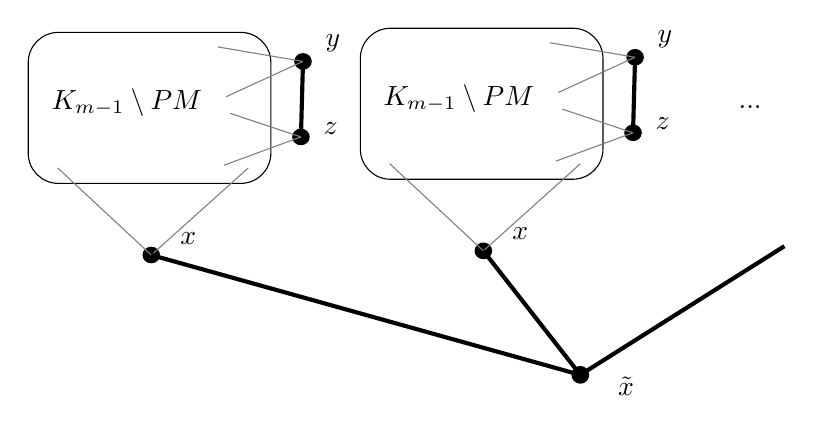
\begin{tikzpicture}[x=0.75pt,y=0.75pt,yscale=-1,xscale=1]
%uncomment if require: \path (0,300); %set diagram left start at 0, and has height of 300

%Rounded Rect [id:dp9473966714969759] 
\draw   (240,35.55) .. controls (240,27.51) and (246.51,21) .. (254.55,21) -- (342.35,21) .. controls (350.39,21) and (356.9,27.51) .. (356.9,35.55) -- (356.9,79.21) .. controls (356.9,87.24) and (350.39,93.76) .. (342.35,93.76) -- (254.55,93.76) .. controls (246.51,93.76) and (240,87.24) .. (240,79.21) -- cycle ;
%Shape: Ellipse [id:dp8001519132009809] 
\draw  [fill={rgb, 255:red, 0; green, 0; blue, 0 }  ,fill opacity=1 ] (295.32,128.27) .. controls (295.32,126.21) and (297.09,124.54) .. (299.28,124.54) .. controls (301.46,124.54) and (303.23,126.21) .. (303.23,128.27) .. controls (303.23,130.33) and (301.46,132) .. (299.28,132) .. controls (297.09,132) and (295.32,130.33) .. (295.32,128.27) -- cycle ;
%Shape: Ellipse [id:dp09533509575608257] 
\draw  [fill={rgb, 255:red, 0; green, 0; blue, 0 }  ,fill opacity=1 ] (367.44,71.37) .. controls (367.44,69.31) and (369.21,67.64) .. (371.39,67.64) .. controls (373.58,67.64) and (375.35,69.31) .. (375.35,71.37) .. controls (375.35,73.43) and (373.58,75.1) .. (371.39,75.1) .. controls (369.21,75.1) and (367.44,73.43) .. (367.44,71.37) -- cycle ;
%Shape: Ellipse [id:dp8692338845146277] 
\draw  [fill={rgb, 255:red, 0; green, 0; blue, 0 }  ,fill opacity=1 ] (368.43,34.99) .. controls (368.43,32.93) and (370.2,31.26) .. (372.38,31.26) .. controls (374.56,31.26) and (376.33,32.93) .. (376.33,34.99) .. controls (376.33,37.05) and (374.56,38.72) .. (372.38,38.72) .. controls (370.2,38.72) and (368.43,37.05) .. (368.43,34.99) -- cycle ;
%Straight Lines [id:da524749265094725] 
\draw [line width=1.5]    (372.38,34.99) -- (371.39,71.37) ;
%Straight Lines [id:da3523205788384721] 
\draw [color={rgb, 255:red, 128; green, 128; blue, 128 }  ,draw opacity=1 ]   (254.16,86.29) -- (299.28,128.27) ;
%Straight Lines [id:da9405791186427831] 
\draw [color={rgb, 255:red, 128; green, 128; blue, 128 }  ,draw opacity=1 ]   (299.28,128.27) -- (346.04,86.29) ;
%Straight Lines [id:da8739071680928246] 
\draw [color={rgb, 255:red, 128; green, 128; blue, 128 }  ,draw opacity=1 ]   (372.38,34.99) -- (331.33,28) ;
%Straight Lines [id:da4300673457322983] 
\draw [color={rgb, 255:red, 128; green, 128; blue, 128 }  ,draw opacity=1 ]   (371.39,71.37) -- (334.33,85) ;
%Straight Lines [id:da8923337233149702] 
\draw [color={rgb, 255:red, 128; green, 128; blue, 128 }  ,draw opacity=1 ]   (372.38,34.99) -- (335.33,52) ;
%Straight Lines [id:da08889663539464732] 
\draw [color={rgb, 255:red, 128; green, 128; blue, 128 }  ,draw opacity=1 ]   (371.39,71.37) -- (337.33,60) ;
%Straight Lines [id:da3884912329496307] 
\draw [line width=1.5]    (299.28,128.27) -- (346,188) ;
%Shape: Circle [id:dp02091061266625116] 
\draw  [fill={rgb, 255:red, 0; green, 0; blue, 0 }  ,fill opacity=1 ] (342,188) .. controls (342,185.79) and (343.79,184) .. (346,184) .. controls (348.21,184) and (350,185.79) .. (350,188) .. controls (350,190.21) and (348.21,192) .. (346,192) .. controls (343.79,192) and (342,190.21) .. (342,188) -- cycle ;
%Rounded Rect [id:dp5228528528747626] 
\draw   (80,37.55) .. controls (80,29.51) and (86.51,23) .. (94.55,23) -- (182.35,23) .. controls (190.39,23) and (196.9,29.51) .. (196.9,37.55) -- (196.9,81.21) .. controls (196.9,89.24) and (190.39,95.76) .. (182.35,95.76) -- (94.55,95.76) .. controls (86.51,95.76) and (80,89.24) .. (80,81.21) -- cycle ;
%Shape: Ellipse [id:dp49878039098437144] 
\draw  [fill={rgb, 255:red, 0; green, 0; blue, 0 }  ,fill opacity=1 ] (135.32,130.27) .. controls (135.32,128.21) and (137.09,126.54) .. (139.28,126.54) .. controls (141.46,126.54) and (143.23,128.21) .. (143.23,130.27) .. controls (143.23,132.33) and (141.46,134) .. (139.28,134) .. controls (137.09,134) and (135.32,132.33) .. (135.32,130.27) -- cycle ;
%Shape: Ellipse [id:dp3515233214082192] 
\draw  [fill={rgb, 255:red, 0; green, 0; blue, 0 }  ,fill opacity=1 ] (207.44,73.37) .. controls (207.44,71.31) and (209.21,69.64) .. (211.39,69.64) .. controls (213.58,69.64) and (215.35,71.31) .. (215.35,73.37) .. controls (215.35,75.43) and (213.58,77.1) .. (211.39,77.1) .. controls (209.21,77.1) and (207.44,75.43) .. (207.44,73.37) -- cycle ;
%Shape: Ellipse [id:dp9274488194012027] 
\draw  [fill={rgb, 255:red, 0; green, 0; blue, 0 }  ,fill opacity=1 ] (208.43,36.99) .. controls (208.43,34.93) and (210.2,33.26) .. (212.38,33.26) .. controls (214.56,33.26) and (216.33,34.93) .. (216.33,36.99) .. controls (216.33,39.05) and (214.56,40.72) .. (212.38,40.72) .. controls (210.2,40.72) and (208.43,39.05) .. (208.43,36.99) -- cycle ;
%Straight Lines [id:da16981621840848482] 
\draw [line width=1.5]    (212.38,36.99) -- (211.39,73.37) ;
%Straight Lines [id:da5933465042171406] 
\draw [color={rgb, 255:red, 128; green, 128; blue, 128 }  ,draw opacity=1 ]   (94.16,88.29) -- (139.28,130.27) ;
%Straight Lines [id:da9882619121692495] 
\draw [color={rgb, 255:red, 128; green, 128; blue, 128 }  ,draw opacity=1 ]   (139.28,130.27) -- (186.04,88.29) ;
%Straight Lines [id:da1625402203407108] 
\draw [color={rgb, 255:red, 128; green, 128; blue, 128 }  ,draw opacity=1 ]   (212.38,36.99) -- (171.33,30) ;
%Straight Lines [id:da8874312547808512] 
\draw [color={rgb, 255:red, 128; green, 128; blue, 128 }  ,draw opacity=1 ]   (211.39,73.37) -- (174.33,87) ;
%Straight Lines [id:da4150754182725327] 
\draw [color={rgb, 255:red, 128; green, 128; blue, 128 }  ,draw opacity=1 ]   (212.38,36.99) -- (175.33,54) ;
%Straight Lines [id:da40846710035553246] 
\draw [color={rgb, 255:red, 128; green, 128; blue, 128 }  ,draw opacity=1 ]   (211.39,73.37) -- (177.33,62) ;
%Straight Lines [id:da9509723537256172] 
\draw [line width=1.5]    (139.28,130.27) -- (346,188) ;
%Straight Lines [id:da17020226129551652] 
\draw [color={rgb, 255:red, 0; green, 0; blue, 0 }  ,draw opacity=1 ][line width=1.5]    (346,188) -- (444.33,126) ;

% Text Node
\draw (363,188) node [anchor=north west][inner sep=0.75pt]   [align=left] {$\displaystyle \tilde{x}$};
% Text Node
\draw (421,57) node [anchor=north west][inner sep=0.75pt]   [align=left] {...};
% Text Node
\draw (312,116) node [anchor=north west][inner sep=0.75pt]   [align=left] {$\displaystyle x$};
% Text Node
\draw (381,63) node [anchor=north west][inner sep=0.75pt]   [align=left] {$\displaystyle z$};
% Text Node
\draw (382,21) node [anchor=north west][inner sep=0.75pt]   [align=left] {$\displaystyle y$};
% Text Node
\draw (250,47) node [anchor=north west][inner sep=0.75pt]   [align=left] {$\displaystyle K_{m-1} \setminus PM$};
% Text Node
\draw (152,118) node [anchor=north west][inner sep=0.75pt]   [align=left] {$\displaystyle x$};
% Text Node
\draw (221,65) node [anchor=north west][inner sep=0.75pt]   [align=left] {$\displaystyle z$};
% Text Node
\draw (222,23) node [anchor=north west][inner sep=0.75pt]   [align=left] {$\displaystyle y$};
% Text Node
\draw (90,49) node [anchor=north west][inner sep=0.75pt]   [align=left] {$\displaystyle K_{m-1} \setminus PM$};


\end{tikzpicture}

    \caption{The construction of $H$.}
    \label{fig:construction-tight}
\end{figure}

\paragraph{Statement about the use of AI}
The authors acknowledge the use of AI tools for polishing this paper, and note that all of the proof ideas were entirely human-generated.

\bibliographystyle{plain}
\bibliography{perc}
\end{document}
